%% include header:
\usetheme{metropolis}
\usepackage{appendixnumberbeamer}

\usepackage{booktabs}
\usepackage[scale=2]{ccicons}

\usepackage{pgfplots}
\usepgfplotslibrary{dateplot}

\usepackage{xspace}
\newcommand{\themename}{\textbf{\textsc{metropolis}}\xspace}

\usepackage[english]{babel}
\usepackage{dsfont}
\usepackage{amsmath}
\usepackage{amssymb}
\usepackage{amsthm}
\usepackage{amsfonts}


%% Define theme color(s):
%% ---------------------------------------------------------------

\usepackage{xcolor}

\definecolor{metropolis_theme_color}{RGB}{35,55,59}
% \definecolor{metropolis_theme_color}{RGB}{110, 117, 87}

%% Color custimzations:
\definecolor{blue}{RGB}{0,155,164}
\definecolor{lime}{RGB}{175,202,11}
\definecolor{green}{RGB}{0,137,62}
\definecolor{titleblue}{RGB}{112,122,82}
\definecolor{deepskyblue}{RGB}{0,191,255}
\definecolor{mygrey}{RGB}{240,240,240}

% \setbeamercolor{progress bar}{fg=deepskyblue}
% \setbeamercolor{frametitle}{bg=metropolis_theme_color}

%% Shaded for nicer code highlighting:
%% ---------------------------------------------------------------

\usepackage{mdframed}
% \usepackage{verbatim}

% Define Shaded if not defined:
\makeatletter
\@ifundefined{Shaded}{%
  \newenvironment{Shaded}{\begin{snugshade}}{\end{snugshade}}%
}{}
\makeatother

\renewenvironment{Shaded}{
  \begin{mdframed}[
    backgroundcolor=mygrey,
    linecolor=metropolis_theme_color,
    rightline=false,
		leftline=false
  ]}{
  \end{mdframed}
}

%% Title Image:
%% ---------------------------------------------------------------

% Load transparent:
\usepackage{transparent}

% Add titlegraphic:
\titlegraphic{
  \vspace{2cm}
  \hspace{5.03cm}
  \transparent{0.2}
  
\includegraphics[width=8cm]{images/logos/LMU}
}

%% Adjust frame number to be displayd as i/n:
%% ---------------------------------------------------------------
\setbeamertemplate{frame numbering}{%
  \insertframenumber{}/\inserttotalframenumber
}
\makeatother


%% Include latex-math:
%% ---------------------------------------------------------------
% Include latex-math
\DeclareOldFontCommand{\sf}{\normalfont\sffamily}{\mathsf}

\IfFileExists{./latex-math/basic-math.tex}{
  \input{./latex-math/basic-math.tex}
  \input{./latex-math/ml-bagging.tex}
  \input{./latex-math/ml-boosting.tex}
  \input{./latex-math/ml-gp.tex}
  \input{./latex-math/ml-mbo.tex}
  \input{./latex-math/ml-nn.tex}
  \input{./latex-math/ml-svm.tex}
  \input{./latex-math/ml-trees.tex}
}{
  \IfFileExists{./../latex-math/basic-math.tex}{
    \input{./../latex-math/basic-math.tex}
    \input{./../latex-math/basic-ml.tex}
    \input{./../latex-math/ml-bagging.tex}
    \input{./../latex-math/ml-boosting.tex}
    \input{./../latex-math/ml-gp.tex}
    \input{./../latex-math/ml-mbo.tex}
    \input{./../latex-math/ml-nn.tex}
    \input{./../latex-math/ml-svm.tex}
    \input{./../latex-math/ml-trees.tex}
  }{}
}

%% Style URLs
%% ---------------------------------------------------------------

\usepackage{hyperref}

\definecolor{myorange}{RGB}{225, 127, 0}
\renewcommand\UrlFont{\color{myorange}}

%% include template:
%% Footer:
\usepackage{xfrac}
\usepackage{framed, color}

\setbeamertemplate{footline}[text line]{%
    \noindent\hspace*{\dimexpr-\oddsidemargin-1in\relax}%
     \colorbox{metropolis_theme_color}{
     \makebox[\dimexpr\paperwidth-2\fboxsep\relax]{
     \color{mygrey}
     \begin{minipage}{0.33\linewidth}
       \secname
     \end{minipage}\hfill
     \begin{minipage}{0.33\linewidth}
       \centering
       \insertshortauthor
     \end{minipage}\hfill
     \begin{minipage}{0.33\linewidth}
       \flushright
       \insertframenumber{}/\inserttotalframenumber
     \end{minipage}     
     }}%
  \hspace*{-\paperwidth}
}


%% Title:
%% ----------------------------------------

\title{Compboost}
\subtitle{Modular framework for component-wise boosting}
\date{\today}
\author{Daniel Schalk}
\institute{LMU Munich\\Working Group Computational Statistics}

%% Wrap Shaded around Shunk to have a nices R output:
%% --------------------------------------------------

% Include before begin document to have Schunk:
\usepackage{Sweave}

\let\OldSchunk\Schunk
\let\endOldSchunk\endSchunk

\renewenvironment{Schunk}
 {\small\begin{Shaded}\OldSchunk}
 {\endOldSchunk\end{Shaded}\normalsize}

%% Prevent code from printing over margin:
%% --------------------------------------------------
 

%% Content:
%% ----------------------------------------

\begin{document}
\Sconcordance{concordance:demo_slides.tex:demo_slides.Rnw:%
1 31 1 1 4 15 1}
\Sconcordance{concordance:demo_slides.tex:./chapters/intro.Rnw:ofs 48:%
1 10 1 1 2 8 0 1 2 8 1 1 5 1 2 11 1}
\Sconcordance{concordance:demo_slides.tex:demo_slides.Rnw:ofs 90:%
53 1 1}
\Sconcordance{concordance:demo_slides.tex:./chapters/latex_math.Rnw:ofs 92:%
1 19 1}
\Sconcordance{concordance:demo_slides.tex:demo_slides.Rnw:ofs 112:%
56 7 1}


\maketitle

\begin{frame}[plain]{Table of contents}
	\setbeamertemplate{section in toc}[sections numbered]
	\tableofcontents[hideallsubsections]
\end{frame}


\section{About the Template}
\begin{frame}[fragile]{Manual Code Chunks}

\begin{figure}
\centering
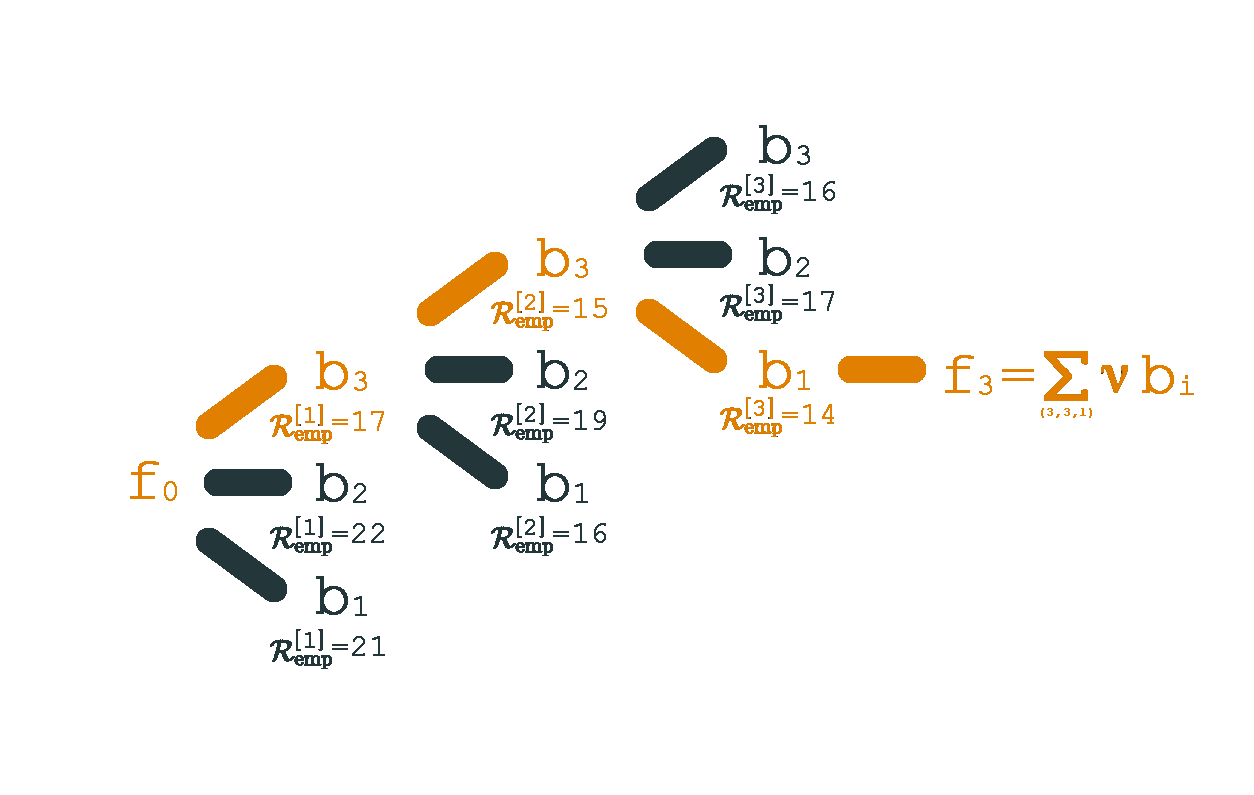
\includegraphics[width=0.7\textwidth]{images/comp_boosting.png}
\end{figure}

\end{frame}

\begin{frame}[fragile]{R Code Chunks}

\begin{Schunk}
\begin{Sinput}
> rnorm(10)
\end{Sinput}
\begin{Soutput}
 [1] -0.03864  0.23352 -0.76209  0.61107 -1.11515  1.25164
 [7]  0.35639  1.40238 -0.01200 -0.27966
\end{Soutput}
\end{Schunk}

\end{frame}

\begin{frame}[fragile]{R Plot Chunks}

To include a \alert{centered plot}, \texttt{Sweave} you need to wrap
\texttt{center} environment:

\begin{center}
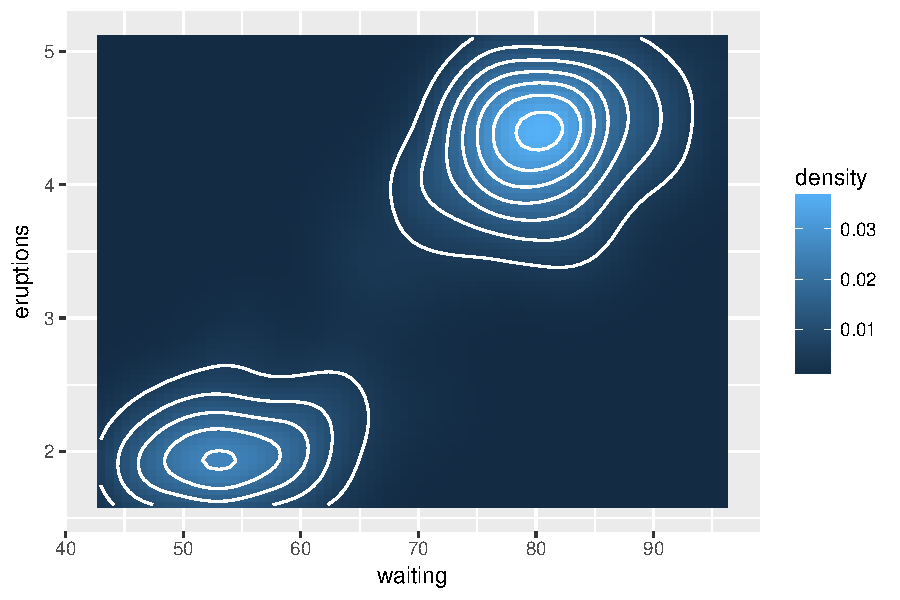
\includegraphics{demo_slides-003}
\end{center}

\end{frame}

\begin{frame}{URLs}

URLs can be easily included by \texttt{\textbackslash url\{myurl\}} and are illustrated in
orange:
\begin{center}
  \url{https://mlr-org.github.io/mlr-tutorial/devel/html/}
\end{center}
\end{frame}

\section{Include latex-math}
\begin{frame}[fragile]{Setting Up Latex-Math}

All you need to do is to clone the \texttt{latex-math} repository into
\texttt{./latex\_pres}:
\begin{verbatim}
git clone http://www.github.com/compstat-lmu/latex-math
\end{verbatim}

\alert{Note:} If you do not have cloned the repo the code should also compile.
Anyway, you then are not able to use \texttt{latex-math}, obviously.

\end{frame}

\begin{frame}{Latex-Math in Action}

\[
\thetah = \argmin_{\theta \in \Theta} \sumin \Lxyi
\]

\end{frame}


\begin{frame}[plain, standout]
  Questions?
\end{frame}


\end{document}
